\section{Создание программного средства} % (fold)
\label{sec:arch_and_mod}

\subsection{Описание классов, атрибутов и методов}
\label{sub:arch_and_mod:graphlib}

Перед началом создания мобильного программного средства необходимо определить список используемых языков программирования, библиотек и технологий, которые будут использоваться для написания приложения.

Для разработки мобильного программного средства, реализуемого в ходе данного дипломного проекта, выбран язык программирования JavaScript. Причина выбора обусловлена некоторыми факторами.

JavaScript является на текущий момент самым высокоразвивающимся и популярным языком программирования. Он имеет очень большое сообщество разработчиков, которые постоянно создают новые библиотеки и дополняют тем самым сам язык и его возможности.

JavaScript является однопоточным языком программирования и это тоже является плюсом. Во-первых, если необходимо распораллеливания определенных функций можно применять асинхронность, которая очень хорошо развита в данном языке программирования, во-вторых, нет необходимости создавать отдельный поток или брать из пула-потоков каждый раз, когда необходимо сделать определенного рода запрос.

JavaScript является мультипарадигменным языком, что позволяет реализовать функции различными способами. Есть возможность использовать объектно-ориентированную парадигму, так и функциональный подход. JavaScript не является функциональным языком программирования, однако, он содержит огромное количество свойств пресущих функциональным языкам:

\begin{itemize}
  \item функции являются объектами высшего порядка;
  \item функции являются объектами высшего порядка;
  \item работа с асинхроностью;
  \item частичное применение функций (carring);
  \item композиция функций (carring).
\end{itemize}

В ходе дипломного проета используется именно фунциональный подход, так как он является более производительным и легко тестируемым. Однако кроме нативного языка используются и дополнительные платформы, библиотеки и фреймворки.

Чтобы JavaScript можно было использовать для разработки мобильного приложения используется платформа Cordova. Cordova позволяет без знания нативной разработки под мобильные телефоны, использовать: JavaScript, HTML, CSS, которые впоследующем компилирует и переводит в машинные команды для определенных видов мобильных операционных систем. 

Суть самой платформы -- встраивание браузера WebView в мобильное приложение. По умолчанию Cordova представляет базовые функции браузера, однако функциональность можно расширить, путем добавления плагинов. Каждый плагин содержит в себе унифицированный интерфейс, позволяющий работать с определенной функциональностью. 

В дипломном проекте используются два плагина:
\begin{itemize}
  \item Плагин для работы с камерой телефона;
  \item Плагин добавляющий в браузер спиннер-загрузки.
\end{itemize}

Для разработки клиентской части приложения  будут использованы следующие библиотеки:
\begin{enumerate}
\item ReactJS;
\item ImmutableJS;
\item Tesseract;
\item Mocha.
\end{enumerate}

ReactJS -- библеотека построеная на концепции компонентов. В основе ReactJS лежит парадигма реактивного программирования. Данная парадигма позволяет описывать данные в виде набора некоторых утверждений или формул. Также создатели React полностью переработали идеалогию работы с DOM элементами. Была реализована новая работа с DOM назыающаяся теневой DOM. Фреймворк использует ее, чтобы при изменении состояния компонента судить о том, что поменять необходимо в реальном DOM и как это сделать наиболее эффективно.

ImmutableJS -- библиотека позволяющая сделать неизменняемые объекты, листы или массивы. Неизменяемость -- основной принцип функционального программирования.

Tesseract -- библиотека для считывания информации с изображений.

Mocha -- эта библиотека содержит общие функции для тестирования, включая describe и it. Позволяет протестировать клиентскую часть приложения дипломного проекта.

Рассмотрим основные классы и методы клиентской части мобильного-приложения представленного на изображении~\ref{fig:domain:manual_structure:client_class}.

\begin{figure}[ht]
\centering
  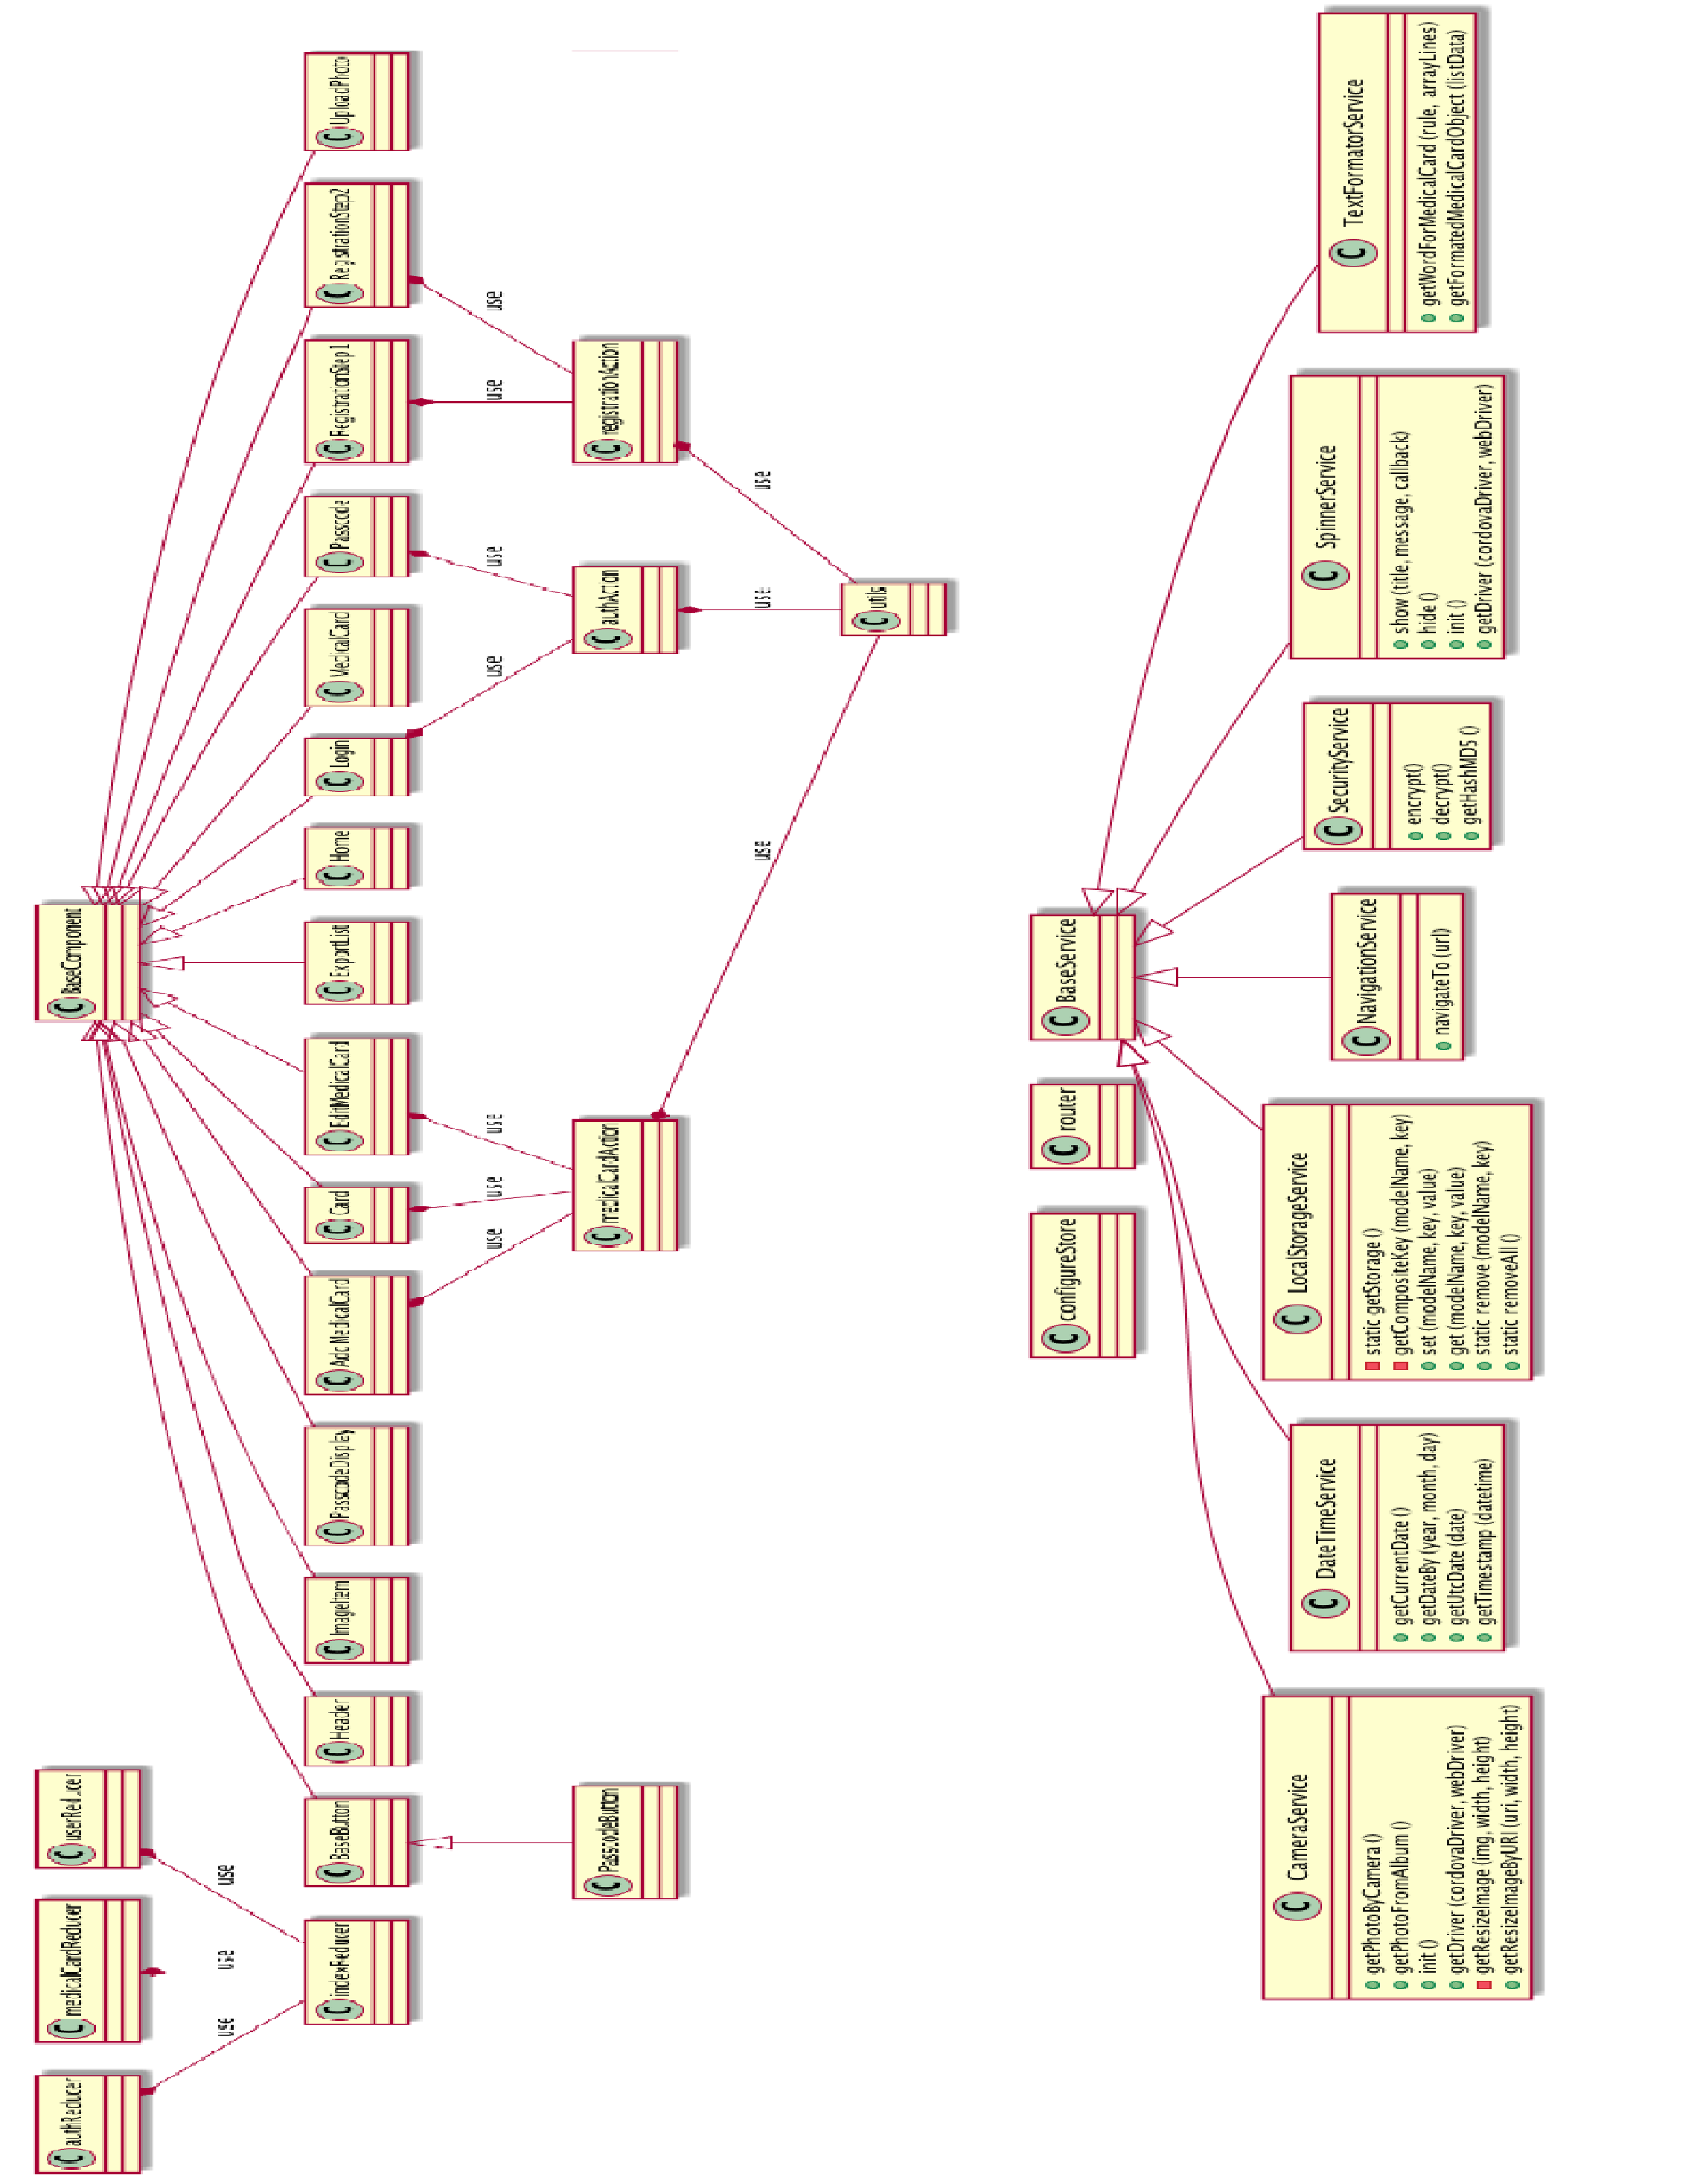
\includegraphics[scale=0.36]{ClassDiagram1.png}  
  \caption{Диаграмма классов компонентов и сервисов}
  \label{fig:domain:manual_structure:client_class}
\end{figure}

Класс ConfigureStore создает и конфигурирует единственное хранилище клиентского-приложения. Содержит единственный метод createStore, который создает хранилище с возможностью отслеживать постоянно его состояние на текущий момент, используется для логинга в приложении.

Класс CordovaCameraDriver создает интерфейс для работы с плагиной CordovaCamera. Содержит одноименные функции плагина: getPicture, distinationType, pictureSourceType. Также содержит в себе метод init, которым производится инициализация данного плагина и его полная конфигурация.

Класс WebCameraDriver создает интерфейс, но уже не для работы с плагином CordovaCamera, а интерфейс для работы с веб-клиентом, так как данное приложение можно будет открыть и на desctop версии, так как оно является кроссплатформенным.

Класс CameraService предоставляет возможность различного рода обработки полученной фотографии от интерфейса CordovaCameraDriver. Основные методы:
\begin{itemize}
  \item getPhotoByCamera достает информацию и саму фотографию, используя интерфейс CordovaCameraDriver;
  \item getResizeImage позволяет изменить размер самой фотографии, до формата, который будет пригоден в дальнейшем использовании;
  \item drawOnCanvas позволяет отрисовать изображение на canvas элементе, для последующей его обработки.
\end{itemize}

Класс LocalStorageService предоставляет возможность работы с браузерным localStorage. Основные методы:
\begin{itemize}
  \item getLocalStorage достает всю информацию из LocalStorage;
  \item getItem позволяет определенный элемент из LocalStorage;
  \item setItem позволяет добавить элемент в LocalStorage;
  \item clear позволяет очистить LocalStorage.
\end{itemize}

Класс SecurityService предоставляет возможность шифрования информации. Использует алгоритм шифрования AES-128 и MD5. Основные методы:
\begin{itemize}
  \item getMD5 достает хэш-функцию, используя алгоритм хэширования MD5;
  \item encrypt шифрует информацию используя алгоритм AES-128;
  \item decrypt дешифрует информацию;
  \item cipher -- тело самого алгоритма шифрования AES-128.
\end{itemize}

Класс TextFormatorService предоставляет возможность создания PDF-документа из JavaScript объекта. Производит парсинг самого объекта используя метод getFormatedMedicalCardObject, который в свою очередь распаршивает информацию полученную с фотографии, представленную в строковом формате. После чего, используя getPDFDocument полученный распаршенный объект сетится в PDF документ.

Классы AuthReducer, MedicalCardReducer, UserReducer представляют собой редьюсеры (чистые функции) для работы с авторизацией или регистрацией, медицинскими карточками, юзером соответственно. В них производится изменение текущего состояния определенного state на новое.

Классы Auth, MedicalCard, Medication, Registration представляют собой Action-объекты, которые содержат в себе обязательное поле типа экшена и второстепенные поля, необходимы для редьюсеров.

Также стоит обратить внимание на определенные функции в компонентах:
\begin{itemize}
  \item takeImport получает изображение, модифицирует его используя фильтры и передает Tesseract библиотеке, которая в свою очередь возвращает распознанный текст с изображения;
  \item handleExport переводит, получаемый объект, в PDF-документ;
  \item setData устанавливает полученные данные с пользовательского ввода в медицинскую карточку, формируя тем самым объект.
\end{itemize}

Каждый компонент содержит несколько обязательных методов. Одним из них является метод render. Он необходим для построения DOM дерева данного представления на основе его шаблона. После построения DOM дерева его корень записывается в атрибут элемента представления.

Метод GetDefaultProps вызывается единожды для класса компонента. Возвращаемый объект используется для свойст по умолчанию, если они не определены родительским компонентом.

Метод GetInitialState вызывается единожды для каждой инстанции компонента, давая возможность инициализировать кастомное состояние каждой инстранции.

Метод componentWillMount вызывается сразу же после начального рендеринга. Это последний момент воздействия на состояние компонента, перед вызовом метода Render.

Метод componentDidMount вызывается при условии, что рендеринг страницы произошел успешно и настоящий DOM срендерен. Тем самым можно произвести некоторое изменения уже на срендеренном элементе.

Рассмотрим основные классы серверной части мобильного-приложения. Класс UserController является базовым контроллером для работы с информацией о пользователе системы. Он содержит все основные методы для работы с пользователем.

Метод register позволяет зарегестрироваться пользователю в системе. В самом методе используется метод валидации, который позволяет отследить введенную пользователем информацию, и, если она содержит не желательную информацию, то метод вернет соответствующую ошибку на клиент и определенный HTTP статус.

Метод login позволяет пользователю авторизоваться в системе, сообщив исходные данные: логин и пароль от своего аккаунта.

Метод addProfile позволяет пользователю добавить более подробную информацию о себе, тут также срабатывает валидация и если пользователь вводит не корректную информацию, сервер вернет ошибку и HTTP статус, сообщая клиентской части, что необходимо предупредить пользователя о неверной информации.

Метод checkPasscode позволяет проверить passcode, который пользователь введет, когда его приложение удалится из памяти. Сделано это для того, чтобы пользователь постоянно не проходил авторизацию, ведь в мобильном телефоне уже осталась информация о том, что он прошел аутентификацию.

Класс medicalCardController -- контроллер для работы с медицинской информацией пользователя. Содержит все основные методы для работы с медицинскими карточками.

\begin{itemize}
  \item addNewCard позволяет добавить новую карточку;
  \item editMedCard позволяет отредактировать выбранную карточку;
  \item setData позволяет удалить выбранную карточку;
  \item addMedication позволяет добавить в медицинскую карточку медикаменты, необходимые для принятия;
  \item addDiagnostic позволяет добавить информацию о диагностике;
  \item getAllMedCard позволяет достать все карточки пациента.
\end{itemize}

Класс cryptoHelper на стороне сервера производит шифрование или дешифрования используя алгоритм AES-256-cbc. Сделано это для того, чтобы была лучшая криптостойкость и чтобы если произойдет взлом криптошифра на стороне клиента, информация на стороне сервера осталась в сохранности, потому что используется уже другой алгоритм. Содержит в себе методы:
\begin{itemize}
  \item encrypt позволяет зашифровать информацию;
  \item decrypt позволяет дешифровать информацию;
  \item createHash позволяет создать новый хэш.
\end{itemize}

Класс validationHelper -- хэлпер для работы с валидацией введенной информацией от пользователя. Содержит в себе методы определения необходимых данных, а также их валидирования, чтобы пользователь не ввел не желательную информацию в систему.

Класс userService производит работу с пользователем на более низком уровне (DAL), производит работу уже непосредственно с объектами-моделями, которые в последующем установятся в базу данных, содержит методы:
\begin{itemize}
  \item registation создает модель нового пользователя и добавляет в базу данных;
  \item login находит пользователя и проверяет введенную им информацию с информацией в базе данных;
  \item checkPasscode находит пользователя и проверяет его пасскод;
  \item addProfile добавляет пользователю дополнительную информацию.
\end{itemize}

Класс medicalService производит работу с медицинскми карточками на уровне DAL, содержит в себе методы:
\begin{itemize}
  \item addMedicalCard создает модель медицинской карточки и заносит ее в базу данных;
  \item editMedicalCard находит определенную медицинскую карточку и изменяет ее в последующем заносит в базу данных;
  \item deleteMedicalCard находит медицинскую карточку и удаляет ее из базы данных;
  \item addDoctorForMedicalCard добавляет к медицинской карточке информацию о враче;
  \item addMedication добавляет к медицинской карточке информацию о медикаментах;
  \item addPaymentInfo добавляет к медицинской карточке информацию о оплате услуг;
  \item getAllMedicalCard достает все возможные медицинские карточки из базы данных.
\end{itemize}

\subsection{Инструкция по сборке ПС}
\label{sub:arch_and_mod:sbor}

\subsubsection{Инструкция и информация по сборке сервера}

Для обеспечения работы сервера необходимо выполнить следующую последовательность действий:
\begin{enumerate}
\item установить сервер NodeJS;
\item установить базу данных MongoDB;
\item выполнить команду npm install, которая установит дополнительные пакеты;
\item проинициализировать базу данных с помощь скрипта mongod;
\item запустить сервер используя команду node server.js.
\end{enumerate}

Для дипломного проекта используется облачный сервис Amazon, который предоставляет масштабируемые вычислительные ресурсы в облаке. На сервере Amazon необходимо произвести конфигурацию, чтобы он имел статический IP-адрес выбранного сервиса. После чего произвести установка операционной системы Ubuntu, после которой можно будет собрать сервер используя команды выше.

\subsubsection{Инструкция по сборке клиентского приложения}

Для обеспечения работы клиентского приложения необходимо выполнить следующую последовательность действий:
\begin{enumerate}
\item установить Java SDK;
\item установить Android Studio;
\item установить XCode;
\item скачать репозиторию Cordova;
\item установить плагины CordovaCamera и SpinnerCordova;
\item выполнить команду npm install, которая установит дополнительные пакеты;
\item выполнить команду cordova run android или cordova run ios.
\end{enumerate}